%% Creator: Inkscape 1.1.2 (b8e25be833, 2022-02-05), www.inkscape.org
%% PDF/EPS/PS + LaTeX output extension by Johan Engelen, 2010
%% Accompanies image file 'DynamicsWT1DOF_Blade.pdf' (pdf, eps, ps)
%%
%% To include the image in your LaTeX document, write
%%   \input{<filename>.pdf_tex}
%%  instead of
%%   \includegraphics{<filename>.pdf}
%% To scale the image, write
%%   \def\svgwidth{<desired width>}
%%   \input{<filename>.pdf_tex}
%%  instead of
%%   \includegraphics[width=<desired width>]{<filename>.pdf}
%%
%% Images with a different path to the parent latex file can
%% be accessed with the `import' package (which may need to be
%% installed) using
%%   \usepackage{import}
%% in the preamble, and then including the image with
%%   \import{<path to file>}{<filename>.pdf_tex}
%% Alternatively, one can specify
%%   \graphicspath{{<path to file>/}}
%% 
%% For more information, please see info/svg-inkscape on CTAN:
%%   http://tug.ctan.org/tex-archive/info/svg-inkscape
%%
\begingroup%
  \makeatletter%
  \providecommand\color[2][]{%
    \errmessage{(Inkscape) Color is used for the text in Inkscape, but the package 'color.sty' is not loaded}%
    \renewcommand\color[2][]{}%
  }%
  \providecommand\transparent[1]{%
    \errmessage{(Inkscape) Transparency is used (non-zero) for the text in Inkscape, but the package 'transparent.sty' is not loaded}%
    \renewcommand\transparent[1]{}%
  }%
  \providecommand\rotatebox[2]{#2}%
  \newcommand*\fsize{\dimexpr\f@size pt\relax}%
  \newcommand*\lineheight[1]{\fontsize{\fsize}{#1\fsize}\selectfont}%
  \ifx\svgwidth\undefined%
    \setlength{\unitlength}{335.96001878bp}%
    \ifx\svgscale\undefined%
      \relax%
    \else%
      \setlength{\unitlength}{\unitlength * \real{\svgscale}}%
    \fi%
  \else%
    \setlength{\unitlength}{\svgwidth}%
  \fi%
  \global\let\svgwidth\undefined%
  \global\let\svgscale\undefined%
  \makeatother%
  \begin{picture}(1,0.57394138)%
    \lineheight{1}%
    \setlength\tabcolsep{0pt}%
    \put(0,0){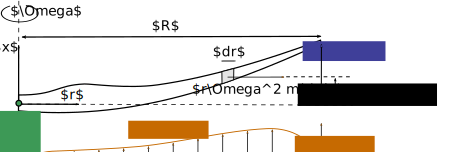
\includegraphics[width=\unitlength,page=1]{DynamicsWT1DOF_Blade.pdf}}%
    \put(0.12456431,0.53677297){\color[rgb]{0,0,0}\makebox(0,0)[t]{\lineheight{0}\smash{\begin{tabular}[t]{c}$\Omega$\end{tabular}}}}%
    \put(0.02802574,0.45095373){\color[rgb]{0,0,0}\makebox(0,0)[t]{\lineheight{0}\smash{\begin{tabular}[t]{c}$x$\end{tabular}}}}%
    \put(0,0){\includegraphics[width=\unitlength,page=2]{DynamicsWT1DOF_Blade.pdf}}%
    \put(0.41031723,0.50153202){\color[rgb]{0,0,0}\makebox(0,0)[t]{\lineheight{0}\smash{\begin{tabular}[t]{c}$R$\end{tabular}}}}%
    \put(0.19157624,0.3414852){\color[rgb]{0,0,0}\makebox(0,0)[t]{\lineheight{0}\smash{\begin{tabular}[t]{c}$r$\end{tabular}}}}%
    \put(0,0){\includegraphics[width=\unitlength,page=3]{DynamicsWT1DOF_Blade.pdf}}%
    \put(0.72971291,0.37467192){\color[rgb]{0,0,0}\makebox(0,0)[lt]{\begin{minipage}{0.3324181\unitlength}\centering $\Phi(r)q(t)$\end{minipage}}}%
    \put(0,0){\includegraphics[width=\unitlength,page=4]{DynamicsWT1DOF_Blade.pdf}}%
    \put(0.65280575,0.34994307){\color[rgb]{0,0,0}\makebox(0,0)[t]{\lineheight{0}\smash{\begin{tabular}[t]{c}$r\Omega^2 m(r) dr$\end{tabular}}}}%
    \put(0,0){\includegraphics[width=\unitlength,page=5]{DynamicsWT1DOF_Blade.pdf}}%
    \put(0.56192558,0.43979692){\color[rgb]{0,0,0}\makebox(0,0)[t]{\lineheight{0}\smash{\begin{tabular}[t]{c}$dr$\end{tabular}}}}%
    \put(0,0){\includegraphics[width=\unitlength,page=6]{DynamicsWT1DOF_Blade.pdf}}%
    \put(0.32056881,0.28575323){\color[rgb]{0.77647059,0.41568627,0.00392157}\makebox(0,0)[lt]{\begin{minipage}{0.19174467\unitlength}\centering $p_x(r,t)$ \end{minipage}}}%
    \put(0,0){\includegraphics[width=\unitlength,page=7]{DynamicsWT1DOF_Blade.pdf}}%
    \put(0.7182112,0.24952359){\color[rgb]{0.77647059,0.41568627,0.00392157}\makebox(0,0)[lt]{\begin{minipage}{0.19063282\unitlength}\centering $f_{e}$ \end{minipage}}}%
    \put(0,0){\includegraphics[width=\unitlength,page=8]{DynamicsWT1DOF_Blade.pdf}}%
    \put(-0.0212298,0.30915072){\color[rgb]{0.23921569,0.6,0.3372549}\makebox(0,0)[lt]{\begin{minipage}{0.13283015\unitlength}\centering B\end{minipage}}}%
    \put(-0.53627281,3.04727907){\color[rgb]{0,0,0}\makebox(0,0)[lt]{\begin{minipage}{0.11055736\unitlength}\end{minipage}}}%
    \put(0.73694483,0.47551605){\color[rgb]{0.24705882,0.24705882,0.6}\makebox(0,0)[lt]{\begin{minipage}{0.19770816\unitlength}\centering $q(t)$\end{minipage}}}%
    \put(0,0){\includegraphics[width=\unitlength,page=9]{DynamicsWT1DOF_Blade.pdf}}%
    \put(0.80639588,0.05959453){\color[rgb]{0,0,0}\makebox(0,0)[t]{\lineheight{0}\smash{\begin{tabular}[t]{c}$1$\end{tabular}}}}%
    \put(0.3025494,0.08382305){\color[rgb]{0,0,0}\makebox(0,0)[lt]{\begin{minipage}{0.3324181\unitlength}\centering $\Phi(r)$\end{minipage}}}%
    \put(0.03249055,0.14630441){\color[rgb]{0,0,0}\makebox(0,0)[t]{\lineheight{0}\smash{\begin{tabular}[t]{c}$x$\end{tabular}}}}%
    \put(0.18331073,0.03567724){\color[rgb]{0,0,0}\makebox(0,0)[t]{\lineheight{0}\smash{\begin{tabular}[t]{c}$r$\end{tabular}}}}%
    \put(0,0){\includegraphics[width=\unitlength,page=10]{DynamicsWT1DOF_Blade.pdf}}%
  \end{picture}%
\endgroup%
